%=============================================================================%
% Author: 	Bram Kuijper
% Date: 	20/03/2019
% Title: 	Python workshop: strings and regex
%=============================================================================%

%=============================================================================%
% Preamble
%=============================================================================%
% Libraries

\documentclass[xcolor=table]{beamer}
\usepackage{beamerthemeshadow}
\usepackage[T1]{fontenc}
\usepackage{helvet}
\usepackage[]{graphicx}
\usepackage{array}
\usepackage{color}
\definecolor{dkgreen}{rgb}{0,0.6,0}
\definecolor{gray}{rgb}{0.5,0.5,0.5}
\definecolor{mauve}{rgb}{0.58,0,0.82}
\definecolor{deepblue}{rgb}{0,0,0.5}
\definecolor{deepred}{rgb}{0.6,0,0}
\definecolor{deepgreen}{rgb}{0,0.5,0}
\definecolor{lightgray}{rgb}{0.92,0.92,0.92}
\usepackage{listings} % to insert code
\usepackage{textpos} % textblock
\usepackage{textcomp} % textblock
\usepackage{hyperref}
\hypersetup{colorlinks=true, urlcolor=blue, linkcolor=black} 
% Listing set up
% bash
\lstdefinestyle{bash}{
language=bash,                     % the language of the code
basicstyle=\scriptsize\ttfamily,       % the size of the fonts that are used for the code
numbers=none,%left,                   % where to put the line-numbers
numberstyle=\tiny\color{gray},  % the style that is used for the line-numbers
stepnumber=1,                   % the step between two line-numbers. If it's 1, each line
                          % will be numbered
numbersep=5pt,                  % how far the line-numbers are from the code
backgroundcolor=\color{lightgray},  % choose the background color. You must add \usepackage{color}
showspaces=false,               % show spaces adding particular underscores
showstringspaces=false,         % underline spaces within strings
showtabs=false,                 % show tabs within strings adding particular underscores
frame=lines,%single,                   % adds a frame around the code
rulecolor=\color{black},        % if not set, the frame-color may be changed on line-breaks within not-black text (e.g. commens (green here))
tabsize=2,                      % sets default tabsize to 2 spaces
captionpos=b,                   % sets the caption-position to bottom
breaklines=true,                % sets automatic line breaking
breakatwhitespace=false,        % sets if automatic breaks should only happen at whitespace
title=\lstname,                 % show the filename of files included with \lstinputlisting;
                          % also try caption instead of title
keywordstyle=\color{blue},      % keyword style
commentstyle=\color{dkgreen},   % comment style
stringstyle=\color{mauve},      % string literal style
escapeinside={\%*}{*)},         % if you want to add a comment within your code
morekeywords={}            % if you want to add more keywords to the set
}

% Python
\lstdefinestyle{python}{
language=python,
formfeed=\newpage,
basicstyle=\scriptsize\ttfamily,
commentstyle=\color{deepgreen},%\color{gray},
numbers=left,
numberstyle=\tiny\color{gray},
stepnumber=1,
numbersep=5pt,
extendedchars=true,
inputencoding=utf8x,
backgroundcolor=\color{lightgray},%\color{white},
showspaces=false,
showstringspaces=false,
showtabs=false,
frame=lines,
upquote=true,
tabsize=4,
captionpos=b,
breaklines=true,
breakatwhitespace=false,
title=\lstname,
escapeinside=||,
keywordstyle=\color{deepblue},
emphstyle=\color{deepred},
stringstyle=\color{mauve},
literate={ö}{{\"o}}1
       {ä}{{\"a}}1
       {ü}{{\"u}}1
       {ç}{{\c{c}}}1
       {ó}{{\'o}}1
%morekeywords={models, lambda, forms}
}

\graphicspath{ {../img/} }
\title[Python for scientific research]{Python for scientific research}
\subtitle{Pattern matching and text manipulation}
\author{Bram Kuijper}
\institute[]{University of Exeter, Penryn Campus, UK}
\titlegraphic{
\hfill

\includegraphics[width=\textwidth, keepaspectratio]{logo.jpg}}
%=============================================================================%
%=============================================================================%
% Start of Document
%=============================================================================%
%=============================================================================%
\begin{document}

%=============================================================================%
%=============================================================================%
\begin{frame}
\titlepage
\end{frame}

%=============================================================================%
%=============================================================================%
\frame{
    \frametitle{Course Schedule} 
    \begin{itemize}
        \item March 6: The basics of programming in Python
            \begin{itemize}
                \item how to run Python code
                \item data types
                \item flow control
                \item functions and modules
            \end{itemize}
            \pause
        \item Today: Applying Python to simplify your life
            \begin{itemize}
                \item text manipulation
                \item regular expressions
                \item working with files
                \item number crunching with \texttt{numpy} and \texttt{scipy}
                \item making graphs using \texttt{matplotlib}
            \end{itemize}
            \pause
        \item March 27th: Advanced subjects
            \begin{itemize}
                \item working with data using \texttt{pandas}
                \item object-oriented programming
                \item automating tasks in MS-office
                \item image manipulation
                \item working on student-generated problems
            \end{itemize}
    \end{itemize}
}
\begin{frame}{What we've done so far}

	\begin{enumerate}\addtolength{\itemsep}{1\baselineskip}
		\item Declare variables using built-in data types and execute operations
		on them
		\item Use flow control commands to dictate the order in which commands are run
		and when
		\item Encapsulate programs into reusable functions, modules and packages
        \item \textbf{Next:} working with textual data and \emph{pattern matching}
	\end{enumerate}

\end{frame}
%=============================================================================%
%=============================================================================%
\begin{frame}[fragile]
    \frametitle{Basic features of strings}
    First, some \href{https://docs.python.org/3/library/stdtypes.html#text-sequence-type-str}{basic features} of working with strings of text in Python:
        \begin{itemize}
            \item Using quotes within strings:
\begin{lstlisting}[style=python]
str1 = "Text with 'embbeded' single quotes" | \pause |
str2 = 'Text with "embedded" double quotes' | \pause |
str3 = "Text with \"escaped\" double quotes" # Text with "escaped" double quotes 
\end{lstlisting}
\pause
            \item Multiline strings demarcated by triple quotes 
                \pause
\begin{lstlisting}[style=python]
multiline = """This is a 
multiline string""" | \pause |
multiline2 = '''Another
multiline string'''
\end{lstlisting}
        \end{itemize}
\end{frame}
%=============================================================================%
%=============================================================================%
\begin{frame}[fragile]
    \frametitle{String literals}
    Different \href{https://docs.python.org/3/reference/lexical_analysis.html#string-and-bytes-literals}{string literals} identifying different types of string:
\begin{itemize}
    \item By default, any string is \emph{encoded} as \href{https://docs.python.org/3/howto/unicode.html}{UTF-8}, allowing for international characters:
\begin{lstlisting}[style=python]
str_normal = "Let's go to Gijón!" | \pause |
str_normal = u"Let's go to Gijón!" # u-prefix, now redundant (Python2) | \pause |
type(str_normal) # <class 'str'>
\end{lstlisting}
\pause
    \item Byte strings (written as \texttt{b"..."}) only contain \href{https://en.wikipedia.org/wiki/ASCII}{ASCII} characters (no international characters):
\begin{lstlisting}[style=python]
str_ascii = b"Let's go to Gijón!" # Error | \pause |
str_ascii = b"Let's go to Gijon!" # only ASCII | \pause |
type(str_ascii) # <class 'bytes'>
\end{lstlisting}
\pause
\item \href{https://docs.python.org/3/howto/unicode.html}{UTF-8} and \href{https://en.wikipedia.org/wiki/ASCII}{ASCII} are encodings which specify how characters translate into 0s and 1s
\end{itemize}
\end{frame}
\begin{frame}[fragile]
    \frametitle{Example encoding: ASCII}
\begin{center}
	\visible{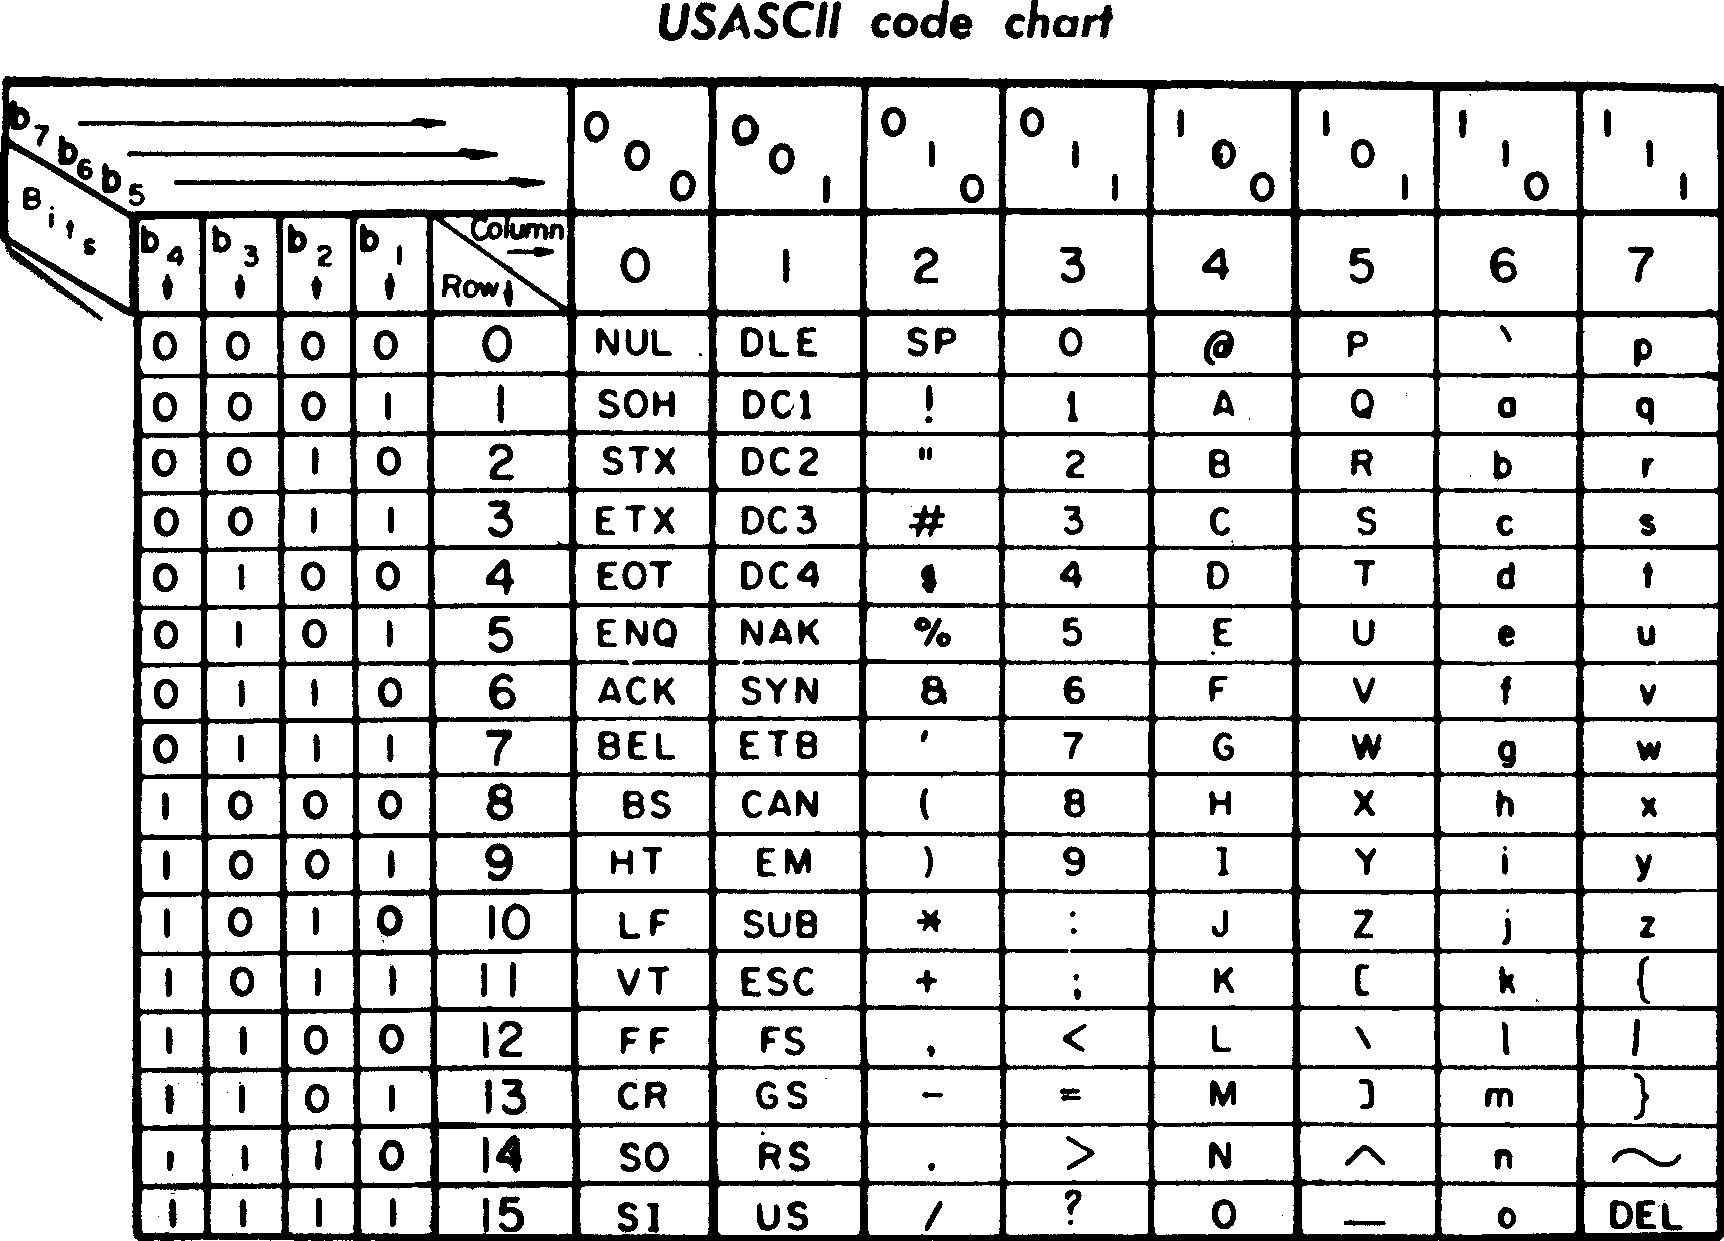
\includegraphics[width=\textwidth]{asciichart.png}}
\end{center}
\end{frame}
\begin{frame}[fragile]
    \frametitle{String literals continued}
\begin{itemize}
    \item International characters sometimes problematic, think web adresses or old filesystems/databases
        \pause
    \item To overcome this, you can use \texttt{str.encode()} to encode into bytes
\begin{lstlisting}[style=python,belowskip=-1.5\baselineskip]
str_var = "Let's go to Gijón!" # utf-8 string | \pause |
str_ascii = str_var.encode() # bytes | \pause |
# b"Let's go to Gij\xc3\xb3n!" | \pause |
\end{lstlisting}
    \item Here, \texttt{\textbackslash xc3} and \texttt{\textbackslash xb3} are \href{https://docs.python.org/3/reference/lexical_analysis.html#grammar-token-stringescapeseq}{escape sequences} that together encode \c{c} as a hex number (see \href{http://www.ltg.ed.ac.uk/~richard/utf-8.cgi?input=&mode=char}{UTF-8} tool) 
        \pause
    \item The original UTF-8 string can be recovered from \texttt{bytes.decode()}
\begin{lstlisting}[style=python]
back_2_utf8 = str_ascii.decode('utf-8') # back to UTF-8
# "Let's go to Gijón!"
\end{lstlisting}
\end{itemize}
\end{frame}

\begin{frame}[fragile]
    \frametitle{Escaping the escape sequences}
\begin{itemize}
    \item Sometimes we do not want \texttt{\textbackslash} to be interpreted as an \href{https://docs.python.org/3/reference/lexical_analysis.html#grammar-token-stringescapeseq}{escape sequence}:
\begin{lstlisting}[style=python,belowskip=-1 \baselineskip] 
windows_path = "C:\new_file.csv"
# C:
# ew_file.csv
\end{lstlisting}
        \pause
\item \texttt{\textbackslash n} is interpreted as a \href{https://en.wikipedia.org/wiki/Newline}{newline character}
    \pause
\item We can prevent this by writing another backslash:
\begin{lstlisting}[style=python,belowskip=-1 \baselineskip]
windows_path = "C:\\new_file.csv"
# C:\new_file.csv
\end{lstlisting} \pause
\item or by using a raw string literal (prefix: \texttt{r"..."})
\begin{lstlisting}[style=python]
windows_path = r"C:\new_file.csv"
# C:\new_file.csv
\end{lstlisting}
\end{itemize}
\end{frame}

\begin{frame}[fragile]
    \frametitle{Various string methods}
    \begin{itemize} 
        \item Lots of \href{https://docs.python.org/3/library/stdtypes.html#string-methods}{string methods} available. Some examples: \pause
    \begin{itemize}\addtolength{\itemsep}{-1\baselineskip}
    \item Split strings in words
\begin{lstlisting}[style=python]
string1 = "Split this string up"
string1.split()
#["Split","this","string","up"]
\end{lstlisting} \pause
    \item Join a list of words
\begin{lstlisting}[style=python]
list_of_words = ["Join","me","together!"]
"--".join(list_of_words)
# Join--me--together!
\end{lstlisting} \pause
    \item Find/replace substrings
\begin{lstlisting}[style=python]
str_subject = "Great rockpools at Swanpool beach"
str_subject.find("pool") # 10
str_subject.rfind("pool") # 23
str_subject.replace("pool","puddle")  # "Great rockpuddles at Swanpuddle beach"
\end{lstlisting} \pause
    \end{itemize} 
\end{itemize} 
\end{frame} 

\begin{frame}[fragile]
    \frametitle{String \texttt{isX} methods}
    \begin{itemize} 
        \item Identifying string contents using various \href{https://docs.python.org/3/library/stdtypes.html#string-methods}{\texttt{str.isX()}} functions \pause
    \begin{itemize}\addtolength{\itemsep}{-1\baselineskip}
    \item All characters in the string are numeric
\begin{lstlisting}[style=python]
string1 = "899898"
string1.isnumeric() # True | \pause |
string2 = "8998.98"
string2.isnumeric() # False
\end{lstlisting} \pause
    \item All characters in the string are alphabetic
\begin{lstlisting}[style=python]
string1 = "Thisisallalphabetic"
string1.isalpha() # True | \pause |
string2 = "Now with whitespace"
string2.isalpha() # False
\end{lstlisting} \pause
    \item Lots of other \texttt{str.isX()} functions available. As we see later, however, regular expressions often preferable to search for patterns in text
    \end{itemize}
\end{itemize}
\end{frame}

%=============================================================================%
%=============================================================================%
\begin{frame}[fragile]
\frametitle{Finding patterns of text without regular expressions}
    \begin{itemize}
        \item Imagine one wants to convert various date formats to YYYY-MM-DD \pause
\begin{lstlisting}[style=python]
s = "23.01.1980,08.09.1990,15-03-2019" | \pause |

for i in range(len(s)):

    if i + 10 <= len(s):
        if s[i:i+2].isdigit() and s[i+2] in ".-" and s[i+3:i+5].isdigit() and s[i+5] in ".-" and s[i+6:i+10].isdigit(): | \pause |
            day = s[i:i+2]
            month = s[i+3:i+5]
            year = s[i+6:i+10]
            print(year + "-" + month + "-" + day)
\end{lstlisting} \pause
\item Gets complicated quickly 
\item Breaks down for single digit months/days, e.g., \texttt{8.9.1980}
    \end{itemize}
\end{frame}

%=============================================================================%
%=============================================================================%
\begin{frame}[fragile]
\frametitle{Finding patterns of text with regular expressions}
\begin{lstlisting}[style=python]
# load the regular expression module
import re | \pause |

# text with dates (with single digit days and months)
s = "23.01.1980,8.9.1990,15-03-2019" | \pause |

# regular expression (given as a r"" [raw literal] string)
all_dates = re.findall(r"(\d{1,2})[-\.](\d{1,2})[-\.](\d{4})",s) | \pause |

# print the result
for date in all_dates:
    print(date[2] + "-" + date[1].zfill(2) + "-" + date[0].zfill(2)) 
\end{lstlisting}
\end{frame}
%=============================================================================%
%=============================================================================%
\begin{frame}[fragile]
\frametitle{What is a regular expression?}
    \begin{itemize}
        \item A tiny, highly specialized programming language within Python \pause 
        \item Made available in the \href{https://docs.python.org/3.7/library/re.html#module-re}{\texttt{re}} module \pause
        \item Specifies the rules to match (and replace) patterns in text \pause 
        \item One line of regex can replace 100s of lines of procedural code \pause 
        \item More portable across different programming languages than \texttt{str} methods \pause 
        \item Easy to create using trial and error, for example on \url{https://regex101.com} \pause 
        \item A simple example:
\begin{lstlisting}[style=python]
import re  | \pause |
str_to_match = "Factors: 1foo, 2foo, foo, 4bar" | \pause |
# regex that matches '1foo', '2foo' etc but not 'foo' | \pause |
regex = r"\dfoo" | \pause |  
re.findall(regex, str_to_match) # ['1foo','2foo']
\end{lstlisting}
    \end{itemize}
\end{frame}

%=============================================================================%
%=============================================================================%
\begin{frame}[fragile]
    \frametitle{Testing regular expressions}
        \begin{itemize}
            \item Practice regular expressions at \url{https://regex101.com/} 
                \begin{center}
	\visible{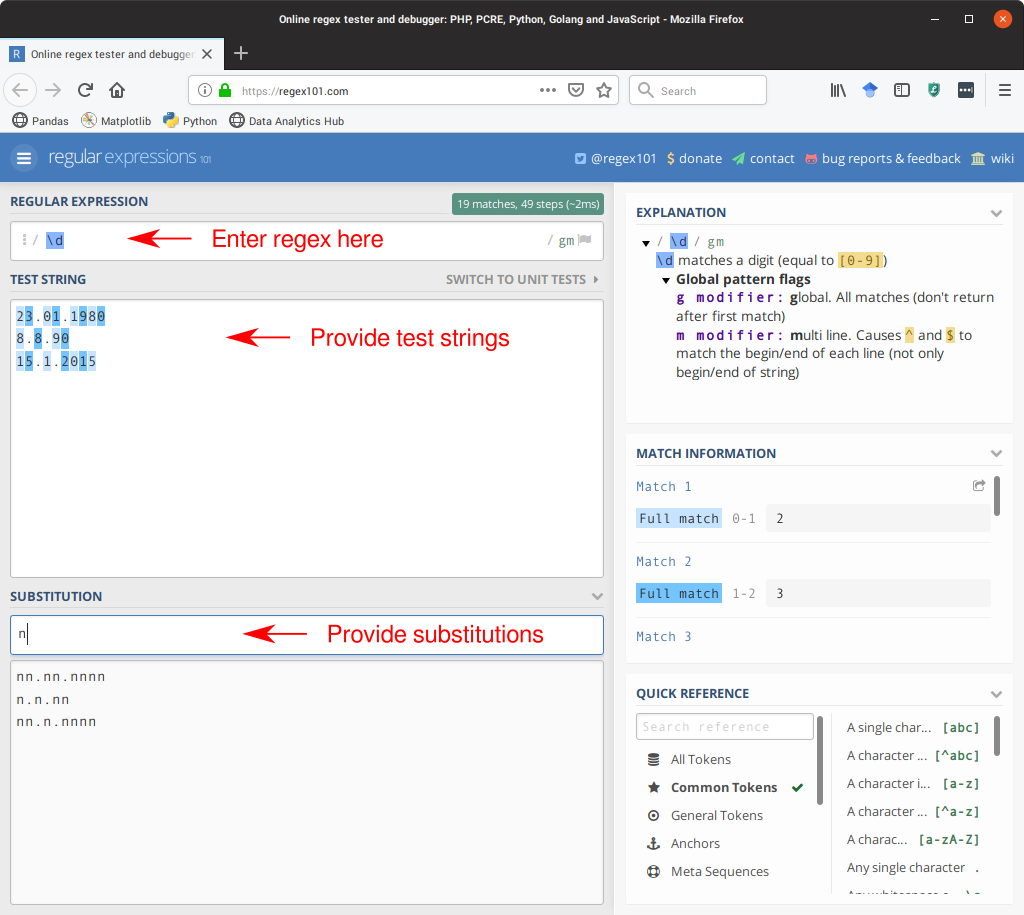
\includegraphics[width=0.7\textwidth]{regex101.png}}
                \end{center}
        \end{itemize}
\end{frame}

%=============================================================================%
%=============================================================================%

\begin{frame}[fragile]
\frametitle{Regular expressions: functions}
    \begin{itemize}
        \item \href{https://docs.python.org/3.7/library/re.html#re.compile}{\texttt{re.compile()}} compiles a regular expression before applying it. Speeds things up when same regex is used a lot of times \pause
        \item \href{https://docs.python.org/3.7/library/re.html#re.findall}{\texttt{re.findall()}} matches all occurrences of a pattern \pause
        \item \href{https://docs.python.org/3.7/library/re.html#re.search}{\texttt{re.search()}} matches the first occurrence of a pattern
\begin{lstlisting}[style=python,belowskip=-1 \baselineskip]
str_to_match = "Factor levels are 1foo, 2foo and foo" | \pause |
# pattern that matches '1foo', '2foo' etc but not 'foo'
regex = r"\dfoo" # regex | \pause |  
m = re.search(regex, str_to_match) # returns a Match object  | \pause |

m.group(0) # '1foo'

regex = r"\dbar" # another regex which does not match | \pause |  
re.search(regex, str_to_match) # None
\end{lstlisting}
    \end{itemize}
\end{frame}

\begin{frame}[fragile]
\frametitle{Regular expressions: functions II}
    \begin{itemize}
        \item \href{https://docs.python.org/3.7/library/re.html#re.sub}{\texttt{re.sub()}} replaces occurrences of patterns in a string \pause
\begin{lstlisting}[style=python,belowskip=-1.5 \baselineskip]
str_to_match = "Factor levels are 1foo, 2foo and foo" | \pause |
# pattern that matches '1foo', '2foo' etc but not 'foo'
# and remembers the digit using a group () 
regex = r"(\d)foo" # regex | \pause |  
# replace foo by bar but keep the digit
replacement = r"\1bar" # regex | \pause |  
re.sub(regex, replacement, str_to_match) # Factor levels are 1bar, 2bar and foo
\end{lstlisting} \pause
        \item Everything within \texttt{()} (a group) is stored in memory \pause
        \item Group contents can be recalled in the replacement, using \texttt{\textbackslash 1},\texttt{\textbackslash 2},\texttt{\textbackslash 3}, etc
    \end{itemize}
\end{frame}
%=============================================================================%
%=============================================================================%

\begin{frame}[fragile]
    \frametitle{Regular expressions: syntax}
    
    The \href{https://docs.python.org/3.7/library/re.html#regular-expression-syntax}{syntax} for different patterns:
    \begin{itemize}
        \item\texttt{\textbackslash d} matches any character that is a digit \pause
        \item\texttt{\textbackslash D} matches any character that is not a digit \pause
        \item\texttt{\textbackslash s} matches any whitespace character (e.g., a space, a tab, a newline) \pause
        \item\texttt{\textbackslash S} matches any character that is not a whitespace \pause
        \item\texttt{\textbackslash b} matches a word boundary \pause
\begin{lstlisting}[style=python,belowskip=-1.5 \baselineskip]
str_to_match = "Factor levels are snafoo, foosna and foo" | \pause |
regex = r"\bfoo\b" # regex | \pause |  
m = re.search(regex, str_to_match) # Factor levels are snafoo, foosna and bar | \pause |
m.group(0) # obtain the complete match | \pause |
m.start() # Match position in string: 37
\end{lstlisting} \pause
        \item\texttt{\textbackslash B} does not match a word boundary 
    \end{itemize}
\end{frame}


%=============================================================================%
%=============================================================================%

\begin{frame}[fragile]
    \frametitle{Regular expressions: syntax II}
    
    The \href{https://docs.python.org/3.7/library/re.html#regular-expression-syntax}{syntax} for different patterns:
    \begin{itemize}
        \item\texttt{.} matches any character (except a newline) \pause
        \item\texttt{\^} matches the start of a string \pause
\begin{lstlisting}[style=python,belowskip=-1.5 \baselineskip]
str1 = "foo snafoo funfoo"
regex = r"^foo" # regex matching the first foo | \pause |  
m = re.search(regex, str1) 
m.start() # match position in string: 0
\end{lstlisting} \pause
        \item\texttt{\$} matches end of a string 
\begin{lstlisting}[style=python,belowskip=-1.5 \baselineskip]
str1 = "foo snafoo funfoo"
regex = r"foo$" # regex matching the last foo | \pause |  
m = re.search(regex, str1) 
m.start() # match position in string: 14 
\end{lstlisting} \pause
    \end{itemize}
\end{frame}
\begin{frame}[fragile]
    \frametitle{Regular expressions: syntax III}
    
    The \href{https://docs.python.org/3.7/library/re.html#regular-expression-syntax}{syntax} for different patterns:
    \begin{itemize}
    \item \texttt{[...]} matches a range of characters
\begin{lstlisting}[style=python,belowskip=-1.5 \baselineskip]
str1 = "the number 60 is larger than 59"
regex = r"[0-5][0-9]" # matches 00 to 59 | \pause |  
m = re.search(regex, str1) 
m.group(0) # '59'
\end{lstlisting} 
    \item \texttt{[\textasciicircum...]} matches characters not in the range 
\begin{lstlisting}[style=python,belowskip=-1.5 \baselineskip]
seq1 = "cccgggtaacccg" | \pause |
regex = r"[^cg]" # do not match c or g | \pause |  
m = re.search(regex, seq1) 
m.group(0)  # 't', first match when using re.search()
\end{lstlisting} 
    \end{itemize}
\end{frame}


%=============================================================================%
%=============================================================================%

\begin{frame}[fragile]
    \frametitle{Regular expressions: repetitions}
    Specify \href{https://docs.python.org/3.7/library/re.html#regular-expression-syntax}{number of times} patterns are matched
    \begin{itemize} \pause
        \item\texttt{*} matches preceding regex 0 or more times \pause
\begin{lstlisting}[style=python,belowskip=-1.5 \baselineskip]
str1 = "numbers 60, 500 and 3000"
regex = r"\d*" # matches 0 or more occurrences of numbers | \pause |  
re.findall(str1,regex) #  ['', '', '', '', '', '', '', '', '60', '', '500', '', '', '', '', '', '3000', '']
\end{lstlisting} \pause
        \item\texttt{+} matches preceding regex 1 or more times \pause
\begin{lstlisting}[style=python,belowskip=-1.5 \baselineskip]
str1 = "numbers 60, 500 and 3000"
regex = r"\d+" # matches 1 or more occurrences of numbers | \pause |  
re.findall(str1,regex) #  ['60', '500', '3000']
\end{lstlisting} \pause
        \item\texttt{?} matches preceding regex 0 or 1 times \pause
\begin{lstlisting}[style=python,belowskip=-1.5 \baselineskip]
str1 = "numbers 60, 500 and 3000"
regex = r"\d?" # matches 0 or 1 occurrences of numbers | \pause |  
re.findall(str1,regex) # ['', '', '', '', '', '', '', '', '6', '0', '', '', '5', '0', '0', '', '', '', '', '', '3', '0', '0', '0', '']
\end{lstlisting} 
    \end{itemize}
\end{frame}

%$
%=============================================================================%
%=============================================================================%
\begin{frame}[fragile]
    \frametitle{Regular expressions: repetitions continued}
    Specify \href{https://docs.python.org/3.7/library/re.html#regular-expression-syntax}{number of times} patterns are matched (continued)
    \begin{itemize} \pause
        \item\texttt{\{n\}} match preceding regex exactly n times \pause
        \item\texttt{\{n,m\}} match preceding regex minimally n and maximally m times \pause
\begin{lstlisting}[style=python,belowskip=-1.5 \baselineskip]
str1 = "numbers 5, 60, 500, 3000, 50000"
regex = r"\d{2,4}" # matches numbers of 2 to 4 digits | \pause |  
re.findall(str1,regex) # ['60', '500', '3000', '5000']
\end{lstlisting} \pause
        \item\texttt{*?}, \texttt{+?}, \texttt{??}, \texttt{\{m,n\}?} minimize the number of times a pattern matches \pause
\begin{lstlisting}[style=python,belowskip=-1.5 \baselineskip]
str1 = "numbers 5, 60, 500, 3000, 50000"
regex = r"\d{2,4}?" # matches numbers of 2 to 4 digits, favoring minimal numbers | \pause |  
re.findall(str1,regex) # ['60', '50', '30', '00', '50', '00']
\end{lstlisting} \pause
    \end{itemize}
\end{frame}

%=============================================================================%
%=============================================================================%

\begin{frame}[fragile]
    \frametitle{Regex exercise}
    \begin{itemize}
        \item Use \url{https://regex101.com/} to write dates in \texttt{"23.01.1980,29-03-2019"} as \texttt{"1980-01-23,2019-03-29"} \pause
        \item Then try to do it in Python \pause 
        \item In Python, that is:
\begin{lstlisting}[style=python,belowskip=-1.5 \baselineskip]
two_dates = "23.01.1980,29-03-2019" 
date_regex = r"(\d{1,2})[\.-](\d{1,2})[\.-](\d{2,4})"
date_substitution = r"\3-\2-\1"
re.sub(date_regex, date_substitution, two_dates)
# 23-01-1980,29-3-2019 
\end{lstlisting} 
    \end{itemize}
\end{frame}

\begin{frame}[fragile]
    \frametitle{Another regex exercise}
    \begin{itemize}
        \item Use \url{https://regex101.com/} to match the words 'pit', 'spot', 'spate', but not 'pt', 'Pot', 'peat', 'part'
\begin{lstlisting} 
    regex = r"s?p(i|o|a)te?"
\end{lstlisting} 
    \end{itemize}
\end{frame}

% End of Document
%=============================================================================%
%=============================================================================%
\end{document}
